\documentclass[12pt]{article}

\usepackage[margin=1in]{geometry}
\usepackage{hyperref}
\usepackage{graphicx}
\usepackage{float}

\hypersetup{
    colorlinks=true,
    urlcolor=blue,  
    linkcolor=blue, 
    citecolor=blue, 
}

\begin{document}

\begin{center}
    {\Large \textbf{Experiment 3 -- TinkerCAD Submission}}
\end{center}

\vspace{0.5em}

\noindent
\textbf{Name:} Manbir Singh Judge \\[0.5em]
\textbf{Roll No.:} 2026113005 \\[0.5em]

\section*{Part A -- Binary Half Adder}

\noindent
\textbf{Tinkercad:}
\href{https://www.tinkercad.com/things/ebDpvZMaMAT-dsm-experiment-3-part-1-and-2?sharecode=TZqAZ21bHZGV4a5mIKK4OJtL0ikV2sPonL3PBrevD4o}{Experiment 3 - Part 1 and 2}

\begin{figure}[H]
\centering

\includegraphics[width=16cm]{1.png}
\caption{Tinkercad Simulation}
\end{figure}

\vspace{0.5em}

\noindent
\textbf{Implementation note:} The half adder was implemented using the standard boolean expressions without any changes.

\vspace{1em}

\section*{Part B -- Binary Full Adder}

\noindent
\textbf{Tinkercad:}
\href{https://www.tinkercad.com/things/ebDpvZMaMAT-dsm-experiment-3-part-1-and-2?sharecode=TZqAZ21bHZGV4a5mIKK4OJtL0ikV2sPonL3PBrevD4o}{Experiment 3 - Part 1 and 2}

\begin{figure}[H]
\centering

\includegraphics[width=16cm]{2.png}
\caption{Tinkercad Simulation}
\end{figure}

\vspace{0.5em}

\noindent
\textbf{Implementation note:} The boolean expression for $C$ (output carry) was modified to avoid using an additional IC for the OR operation. The required OR functionality was implemented using unused gates available in the XOR and AND ICs.

$$
C=C_1 + C_2 = (C_1 \oplus C_2) \oplus (C_1 \cdot C_2)
$$


\vspace{1em}

\section*{Part C -- Binary Half Subtractor}

\noindent
\textbf{Tinkercad:}
\href{https://www.tinkercad.com/things/fnvClRjKQg0-dsm-experiment-3-part-3?sharecode=cYCmQMRLdYlVF9FCfp8gIeCjlj78PSv52U0TRZrD8QU}{Experiment 3 - Part 3}

\begin{figure}[H]
\centering
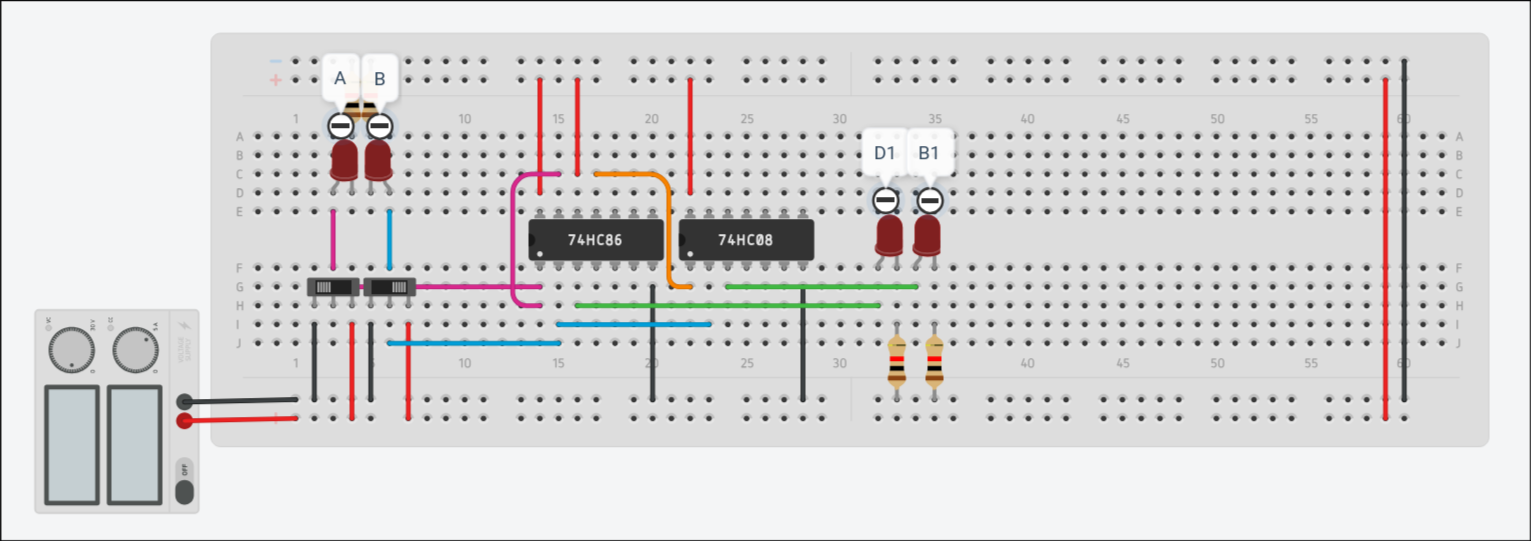
\includegraphics[width=16cm]{3.png}
\caption{Tinkercad Simulation}
\end{figure}

\vspace{0.5em}

\noindent
\textbf{Implementation Note:} Instead of using a separate NOT IC to get the complemented, XOR with logic HIGH was used as follows:

$$
\overline{A}=A\oplus1
$$

\vspace{1em}

\section*{Part D -- Binary Full Subtractor}

\noindent
\textbf{Tinkercad:}
\href{https://www.tinkercad.com/things/d1FqF97gTOR-dsm-experiment-3-part-4?sharecode=CcVcad4-vT3XXqIVOh77uDOH8632an0Vxnek2zZFvnY}{Experiment 3 - Part 4}

\begin{figure}[h]
\centering
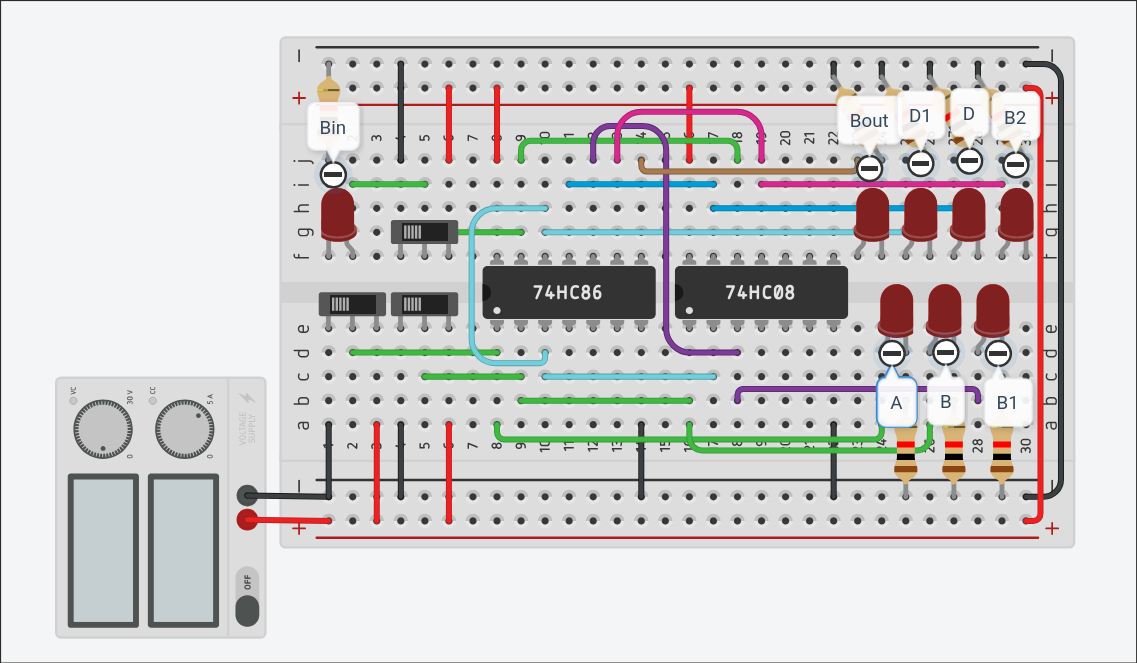
\includegraphics[width=14cm]{4.png}
\caption{Tinkercad Simulation}
\end{figure}

\vspace{0.5em}

\noindent
\textbf{Implementation Note:} The standard boolean expressions were substantially rearranged and simplified to reduce the number of gates and avoid unnecessary additional ICs. The resulting circuit uses the available gates more efficiently while remaining logically equivalent to the full subtractor. Following are the used expressions:
\begin{itemize}
  \item $D_1 = A \oplus B$ \hfill Standard form
  \item $D = D_1 \oplus B_{in}$ \hfill Standard form
  \item $B_1 = B \cdot (A \oplus B) = B \cdot D_1$ \hfill Modified
  \item $B_2 = B_{in} \cdot D$ \hfill Modified
  \item $B_{out} = B_1 \oplus B_2$ \hfill Modified
\end{itemize}
% \begin{itemize}
%   \item $D_1 = A \oplus B$
%   \item $D = D_1 \oplus B_{in}$
%   \item $B_1 = B \cdot (A \oplus B)$
%   \item $B_2 = B_{in} \cdot D$
%   \item $B_{out} = B_1 \oplus B_2$
% \end{itemize}

\vspace{1em}

\end{document}